\documentclass[12pt]{extarticle}
\usepackage[english]{babel}
\usepackage{NotesTeX}
\usepackage{subfigure}
\usepackage{tikz}
\usetikzlibrary{arrows}
\usepackage{multirow}
\usepackage{listings}
\usepackage{extarrows}
\usepackage{parskip}
\usepackage{eurosym}
\usepackage{footmisc}

\graphicspath{{../output/}}
\collaborationImg{
\includegraphics[width=30mm]{../../pictures/UIO.png}}

\author{\Large Vetle Nevland, Vetle Vikenes \& Sigurd Sørlie Rustad}
\title{\Huge Machine Learning: Bra Tittel}
\affiliation{\large FYS-STK4155 – Applied Data Analysis and Machine Learning
\\Autumn 2021\\Department of Physics\\University of Oslo\\\\\today}
\begin{document}
\abstract{Coming soon!
}
\maketitle
\pagestyle{myplain}

\section{Introduction}

We will in no way answer all questions linked to the aforementioned methods. So that anyone can reproduce or continue our studies, we list all the code, results and instructions on running the code in our GitHub repository\footnote{\href{https://github.com/sigurdru/FYS-STK4155/tree/main/project2}{https://github.com/sigurdru/FYS-STK4155/tree/main/project3}}.

\section{Theory}
In the theory-section we aim to give a brief explanation of the main concepts and terminology used in this report. 

\subsection{The diffusion equation}

The full diffusion equation reads
\begin{equation}
\frac{\partial u(\mathbf{r}, t)}{\partial t} = \nabla \cdot \left[D(u, \mathbf{r})\nabla u(\mathbf{r}, t)\right],
\end{equation}
where $\mathbf{r}$ is a positional vector and $D(u,r)$ the collective diffusion coefficient. If $D(u,\mathbf{r}) = 1$ the equation simplifies to a linear differential equation
\begin{equation}
\frac{\partial u}{\partial t} = \nabla^2u(\mathbf{r}, t),
\end{equation}
or
\begin{equation}
\label{eq:diffusion_equation}
\left(\frac{\partial^2}{\partial x^2} + \frac{\partial^2}{\partial y^2} + \frac{\partial^2}{\partial z^2}\right) u(x,y,z,t) = \frac{\partial u(x,y,z,t)}{\partial t}
\end{equation}
in cartesian coordinates. In this report we are going to study a one dimensional rod of length $L=1$. I.e. we need the one dimensional diffusion equation
\begin{align}
\label{eq:diffusion_equation_1D}
\frac{\partial^2 u(x,t)}{\partial x^2} &= \frac{\partial u(x,t)}{\partial t},
\end{align}
with boundary conditions
\begin{align}
u(x,0) &= \sin(\pi x) \ \ 0\leq x\leq L,\\
u(0,t) &= 0 \ \ t\geq 0 \text{ and} \\
u(L,t) &= 0 \ \ t\geq 0.
\end{align}

\subsection{Analytical solution}
An analytical solution of the 1D diffusion equation can be dervied using the method of separation of variables.
\[ u(x,t) = X(x)T(t) \]
The solution is separated into a function $X$ only depending on the independent variable $x$, and a function $T$ only depending on the independent variable $t$. Equation \ref{eq:diffusion_equation_1D} can then be rewritten as

\begin{align*}
	\frac{\partial^2 X(x)T(t)}{\partial x^2} &= \frac{\partial X(x)T(t)}{\partial t} \\
	T(t)\frac{\partial^2 X(x)}{\partial x^2} &= X(x)\frac{\partial T(t)}{\partial t} \\
	\frac{1}{X}\frac{\partial^2 X(x)}{\partial x^2} &= \frac{1}{T}\frac{\partial T(t)}{\partial t}
\end{align*}

The core of the method now becomes clear. The independent variables are separated and put on either side of the equation. Because $x$ and $t$ are independent we may fix one of them, say $x$, while letting the other ($t$) vary. The left side of the equation is thus constant, and since we have equality the expression on the right side must equal the same constant, for arbitrary $t$. Therefore, we can set the left side and right side equal to a constant $-k^2$. The reason for defining a negative constant is to prevent a growing solution, which will be clear on the derivation.

\[ \frac{1}{X}\frac{\partial^2 X(x)}{\partial x^2} = \frac{1}{T}\frac{\partial T(t)}{\partial t} = -k^2\]

This is solved for the functions $X$ and $T$ separately. ...

\subsection*{Explicit forward Euler}
In this section we want to cover the explicit forward Euler. By explicit we mean that the value at the next grid point is determined entirely by known or previously calculated values.

The one-dimensional diffusion equation \eqref{eq:diffusion_equation_1D} reads 
\begin{equation}
\frac{\partial^2u(x, t)}{\partial x^2} = \frac{\partial u(x,t)}{\partial t} \ \ \text{or} \ \ u_{xx} = u_t.
\end{equation}
In this report we are going to study a one dimensional rod of length $L=1$, with boundary conditions
\begin{align}
	u(x,0) &= \sin(\pi x) \ \ 0\leq x\leq L,\\
	u(0,t) &= 0 \ \ t\geq 0 \text{ and} \\
	u(L,t) &= 0 \ \ t\geq 0.
\end{align}

To approximate the solution, we have to discretize the position and time coordinates. We can choose  $\Delta x = L/N$ and $\Delta t$ as small steps in $x$-direction and time, where $N$ are the number of discretized points in $x$-direction. Then we can define the value domain of $t$ and $x$,
\begin{equation*}
t_j = j\Delta t, \ \ j\in \mathbb{N}_0 \ \ \wedge \ \ x_i = i\Delta x, \ \ \{i \in \mathbb{N}_0 | i \leq N\}.
\end{equation*}

The algorithm for explicit forward Euler in one dimension (from \cite{lectures2015} chapter 10.2.1) reads
\begin{equation}
\label{eq:forward_euler}
u_{i, j+1} = \alpha u_{i-1, j} + (1 - 2\alpha) u_{i,j} + \alpha u_{i+1, j}
\end{equation}
where
\begin{equation*}
\alpha = \frac{\Delta t}{\Delta x^2}.
\end{equation*}
This has a local approximate error of $O(\Delta t)$ and $O(\Delta x ^2)$. Experiments show that the following bound on $\alpha$ ensures stability.
\begin{equation}
	\label{eq:stability}
	\alpha = \frac{\Delta t}{\Delta x^2} \le \frac{1}{2}.
\end{equation} 

Even though $\alpha = 0.5$ is at the transition between stable and unstable solutions, experiments show that it is a safe choice for the diffusion equation that produces stable solutions \cite{Linge2017}. Thus, the stability factor $\alpha=0.5$ is used as default in this project. \\ 

We are to use the forward Euler method to discretize the diffusion equation to be solved numerically. The forward Euler is an explicit scheme, meaning that the derivative in time is approximated at the current time level.
That is, the derivative is discretized only by known values. As a consequence, the discretized diffusion equation can be explicitly be solved for the next time step without the need of any matrix inversion to arrive at a coupled
set of discretized equations. The drawback of explicit methods is that it is less stable than implicit schemes, which approximate the derivative at the next time step.
If the derivative is calculated at the current time level, we miss any information about how the solution changes at the next time level. 
Hence, if the gradient of the next time level is significantly different than of the current time level, the numerical solution may deviate considerably from the true solution. 
If the deviation is large enough, further iterations could potentially cause instable solutions in the sense that it diverges.
\par The forward Euler scheme in general requires a quite low time step $\Delta t$ to produce stable solutions. Small time steps are convenient at the start of the diffusion process when the solutions changes quickly. However, when approaching the stationary limit the solution changes very slow and so does the update when using small $\Delta t$. This limitation is resolved by implicit methods \cite{Linge2017}.

\section{Solving Differential equations with deep learning}
Many of the concepts we use in this section is covered in a previous report \cite{project2}. There, in the theory section, we cover central concepts like deep neural networks, cost functions, gradient descent, etc. In this report we will follow closely the work by Maziar Raissi et.al. \cite{raissi2017physics} and this Jupiter-Notebook\footnote{\texttt{https://colab.research.google.com/github/janblechschmidt/PDEsByNNs/blob/main/PINN \_Solver.ipynb\#scrollTo=1PlqQM9aZEkd}}. This method works with any partial differential equation (PDE), however for simplicity we will look at the diffusion equation in one dimension \eqref{eq:diffusion_equation_1D}. 

The idea is that we have some neural network $N$ with parameters $\theta$, including $x$ and $t$ as inputs, and returns $u_{\theta}(x,t)$. After training the neural network, it has found the parameters $\hat{\theta}$ that best approximates its output with the actual solution $u(x,t)$ of the PDE
\begin{align*}
	u_{\hat{\theta}} (x, t) \approx u(x, t).
\end{align*}

The process starts by defining a trial function $u_{\theta}(x,t)$ which is an initial guess of the actual solution $u(x,y)$, defined as

\begin{align}
	u_{\theta}(x,t) = u_0(x, t) + f\big(x, N(x,\theta)\big),
	\label{eq:NN_model}
\end{align}
where $u_0$ is a function specifically designed to satisfy the initial and boundary conditions of the PDE. The function $f$ is the part that is to be optimized by the algorithm. It depends on $x$ and the parameters $\theta$ through the neural network $N$, and should return 0 for the initial and boundary conditions. Constructing the function $f$ should beneficially incorporate prior knowledge about how the solution behaves, because this will accelerate the learning process.

\par We then define the residual $r_\theta(t, x)$, which is the output of the neural network inserted back into the PDE \eqref{eq:diffusion_equation_1D}
\begin{align}
	r_\theta(x, t) \equiv \frac{\partial u_\theta}{\partial t} - \frac{\partial^2 u_\theta}{\partial x^2}.
	\label{eq:residual}
\end{align}

Ideally this should be zero, impying a perfect reproduction of the actual solution. The residual becomes our main object for training, as it gives a measure of how good the neural network approximates the actual solution. For the neural network to improve its predictions a loss function is required, which is to minimized. The sum of squared residuals (across all data samples $n$) serves as an appropriate loss.

\begin{align*}
	L(x, t, \theta) = \sum_{i=1}^n [r_\theta(x_i,t_i)]^2
\end{align*}

Optimization is then done through gradient descent, minimizing the loss with respect to the parameters $\theta$

\begin{align*}
	\theta \leftarrow \theta - \eta \nabla_{\theta}L(x,t,\theta),
\end{align*}

where $\eta$ is the learning rate, which can either be constant or variable - depending on the optimization strategy.
The loss function converges towards zero for the optimal parameters $\theta$, in which case the gradient of the loss function vanishes. As a result, the parameters will hardly update anymore through gradient descent, indicating that we have reached an optimal solution.


\section{Method}
\subsection*{Unit testing}
Before the numerical explicit scheme is applied to a particular problem, it is important to test that the discretized equations return expected results. Unit tests are constructed to test the implementation . This is done by manually calculating the solution of the first two time steps given the initial condition, and comparing the result with that obtained by the numerical scheme. Since the same recursive formula is used for all time steps, it is sufficient to test the two first time steps. To avoid too much computations we choose five equally sized intervals between $x=0$ and $x=L=1$, that is $\Delta x = 0.2$. The time step is set to $\Delta t = 0.01$, ensuring stability.
For the first time step $j=1$, that is $t=\Delta t$, we have the following two boundary values and four interior points

\begin{align*}
	u_0^1 &= u_5^1 = 0 \\
	u_i^1 &= \frac{\Delta t}{\Delta x^2}u_{i+1}^0 + (1 - 2\frac{\Delta t}{\Delta x^2})u_i^0 + \frac{\Delta t}{\Delta x^2}u_{i-1}^0 \\
	&= 0.05u_{i+1}^0 + 0.9u_i^0 + 0.05u_{i-1}^0
\end{align*}

Using the initial condition $u_*^0 = \big(\sin(0),\:\sin(0.2\pi),\:\sin(0.4\pi),\:\sin(0.6\pi), \:\sin(0.8\pi),\:\sin(\pi)\big)$, we get

\begin{align*}
	u_0^1 &= 0 \\
	u_1^1 &= 0.531656755 \\
	u_2^1 &= 0.8602387 \\
	u_3^1 &= 0.8602387 \\
	u_4^1 &= 0.531656755 \\
	u_5^1 &= 0
\end{align*}

The forward euler scheme prints out the following values for the first time step
\[ (0.,\:         0.53165676,\: 0.8602387,\:  0.8602387,\:  0.53165676,\: 0.        ) \]
Hence, the result from forward euler is equal to the manual calulations up to machine precision.

\par Using the values from the first time step, we can calculate the solution at second time step. The recursive formula makes the manual calculations straightforward.

\begin{align*}
	u_0^2 &= 0 \\
	u_1^2 &= 0.480888053 \\
	u_2^2 &= 0.778093215 \\
	u_3^2 &= 0.778093215 \\
	u_4^2 &= 0.480888053 \\
	u_5^2 &= 0
\end{align*}

The forward euler scheme gives the following result for the second time step
\[ (0.,\:         0.48088805,\: 0.77809321,\: 0.77809321,\: 0.48088805,\: 0.        ) \]
Once again, the two approaches provide the same result up to machine precision. Thus, the internal functionality of forward euler is validated. It remains to verify the accuracy of the scheme by comparing it with the analytical solution of the diffusion equation \ref{eq:diffusion_equation_1D} with provided initial and boundary conditions.

\subsection*{Accuracy assessment}
The unit test shows that the forward euler scheme works as expected, but to what accuracy can it reproduce the analytical solution? To address this we compute the deviation of the numerical solution to the analytical solution for two different mesh resolutions in space, $\Delta x=0.1$ and $\Delta x = 0.01$. For comparison purposes the time step is adjusted in each case to ensure stability, and is defined as $\Delta t = 0.5\cdot \Delta x^2$. The error is computed and accumulated for a fixed number of time steps $N$ in both cases. The applied error measure at a given time step is simply the maximum absolute difference between the numerical solution $u$ and the analytical solution $u_e$ across the entire spatial domain.
\[ e^n = \argmax_{i \in [0,N_x]} |u_i^n - u_{e,i}^n| \]

Accounting for the order of accuracy of the forward euler scheme, the error can be expressed as a linear combination of the mesh resolutions $\Delta t$ and $\Delta x$ \cite{Linge2017}

\[ e^n = C_t\Delta t + C_x\Delta x^2 \]

The total accumulated error is given by
\[ E = \sum_{n=1}^N e^n, \]
which is the error measure to be used when testing how well the numerical solution approximates the analytical solution.

\par For the neural network, the total error is given by the sum of squared residuals \ref{eq:residual}. This accumulates the error in the approximated solution for each time step, just as is done for the error in forward euler. As a result, one can make a feasible comparison of the errors.



\section{Results}

\subsection*{Error of Forward Euler scheme}

To assess the accuracy of our implemented numerical scheme, we need to test the how well the produced solution fits the analytical solution. In this project we use the accumulated maximum absolute error, as described in Methods.

\begin{table}[h]
	\centering
	\begin{tabular}{|l|l|l|l|}
		\hline
		\textbf{n}      & \textbf{5} & \textbf{10} & \textbf{50} \\ \hline
		$\Delta x=0.1$  & 0.0061     & 0.0155       & 0.0838       \\ \hline
		$\Delta x=0.01$ & 6.073$\cdot 10^{-5}$      & 1.536$\cdot 10^{-4}$       &   8.302$\cdot 10^{-4}$     \\ \hline
	\end{tabular}
\caption{Accumulated maximum absolute error between numerical solution and analytical solution of the 1D diffusion equation. The test is performed for two different spatial resolutions and for three number of time steps.}
\label{tab:errors}
\end{table}

The test of accumulated error for $\Delta x=0.1$ and $\Delta x=0.01$ for different number of time steps $n$ is shown in Table \ref{tab:errors}. The accumulated error obviously increases when evaluating the error for more time steps because more individual errors are accumulated to the total error. Another feature is that reducing the spatial step $\Delta x$ significantly reduces the accumulated error. For instance, from Table \ref{tab:errors} we have that $0.838/8.302\cdot 10^{-4}=100.94$. Approximately the same factor is reproduced by the other time steps $n$ as well. This shows that reducing $\Delta x$ by a factor of 10 will reduce the accumulated error by a factor of 100. Hence, refining the spatial resolution will significantly improve the performance of the forward euler scheme. The results strongly indicate that the numerical solution converges to the analytical solution as $\Delta x \rightarrow 0$. 

\begin{figure}[h]
	\centering
	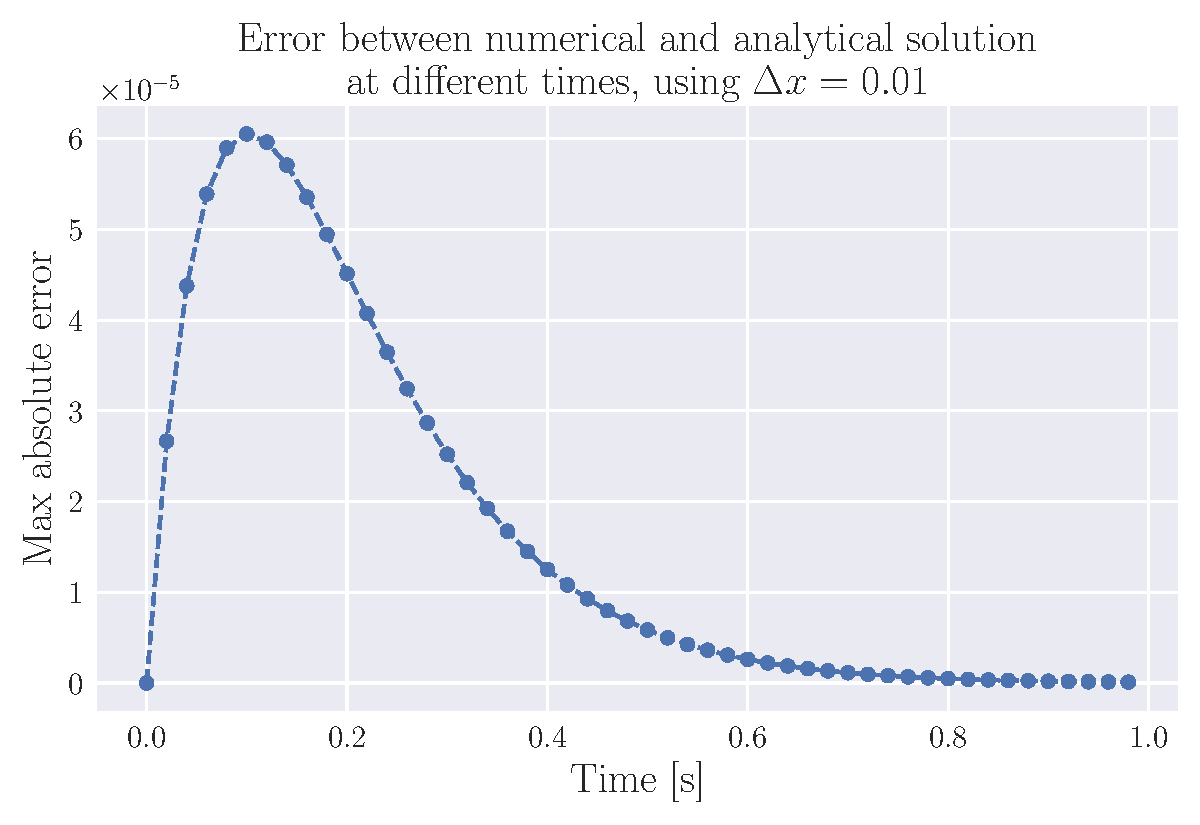
\includegraphics[scale=0.5]{../output/plots/error_FE}
	\caption{Maximum absolute error calculated for 50 uniform time steps from start to end, using $\Delta x=0.01$ and time step $\Delta t$ dictated by the stability criterion \ref{eq:stability}.}
	\label{fig:error_dx001_n50}
\end{figure}

\par A plot of the maximum absolute difference between the numerical and analytical solution for $\Delta x=0.01$ is shown in Figure \ref{fig:error_dx001_n50}. The time step is chosen to give a stability factor $\alpha=0.5$. Notice that the error for time step $n=0$ is zero. This is because the numerical solution for the first time step is simply the initial condition, yielding a perfect correspondance with the analytical solution. As time proceeds, the error quickly increases and reaches a maximum at around time $t=0.1$. This time step is early in the diffusion process, where the solution changes rather quickly. The forward euler scheme is first order accurate in time, $O(\Delta t)$, and second order accurate in space, $O(\Delta x^2)$, implying that the numerical solution is more sensitive to the temporal evolution than the spatial evolution. Hence, the forward euler scheme will produce larger errors for the initial time levels due to the rapid change in solution. At later time stages, after the maximum around $\Delta t=0.1$, the absolute error seems to decrease logarithmically. As the time approaches the end of the simulation, there is hardly any remaining diffusion as the solution is approximately linear. Despite being first order accurate in time, the forward euler scheme is able to reprocude this slowly changing solution with a high accuracy. Figure \ref{fig:error_dx001_n50} verifies this behaviour, illustrating the error converging to zero sufficiently deep into the diffusion process.

\subsection*{Error of Neural Network}

\begin{figure}[h]
	\centering
	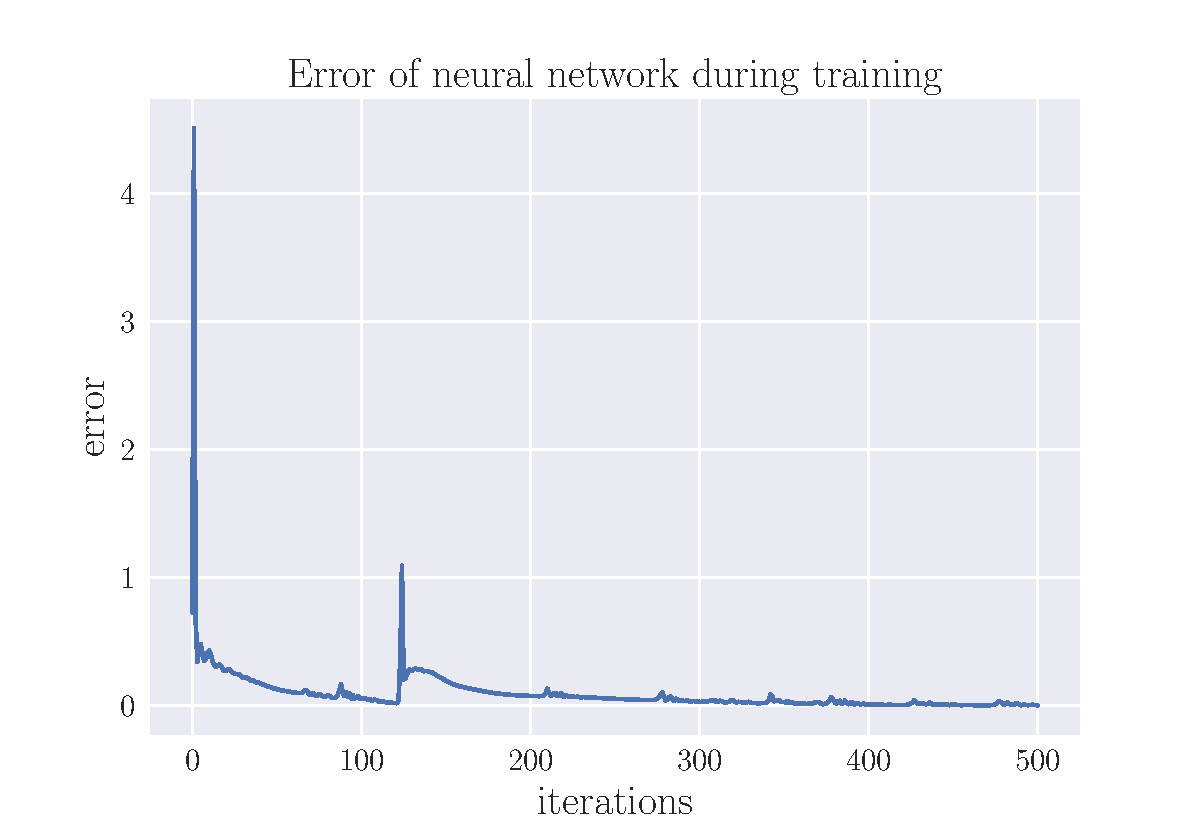
\includegraphics[scale=0.5]{../output/plots/NN_diffusion_error_10000}
	\caption{Residual of approximated solutions to the 1D diffusion equation as function of iterations. The neural network performing 500 iterations, training on 10000 points.}
	\label{fig:error_NN_10000}
\end{figure}

The performance of the neural network is evaluated in a different way than the forward euler discretization scheme. With finite differencing the error is calculated as an absolute difference between the numerical and analytical solution for each time step. For the neural network though, the error during training is calculated by inserting the predicted solution into the abstract form of the differential equation, $F(u)=0$, obtaining a residual $r_{\theta}$. The resulting loss is given by Equation \ref{eq:residual}. Hence, the error of the neural network does not depend on any analytical solution. Figure \ref{fig:error_NN_10000} shows the error of the neural network when approximating the solution $u_{\theta}$ to the actual solution $u$ as a function of training iterations. Initially, the error decreases extremely fast - it reduces by a factor of ten for just a couple of iterations, and the approximated solution improves significantly. Afterwards, the error decreases by a much slower rate with some minor fluctuations. Some time after 100 iterations the error is subject to a large jump, but quickly diminishes agains. For later iterations the error slowly converges towards zero, possessing some irregular, minor fluctuations. 
\par \textcolor{red}{PUT THIS IN DISUSSION?:} The reason that the error flucuates instead of decreasing monotonically is that we use the Adam optimizer [\textcolor{red}{https://arxiv.org/abs/1412.6980}]. This is a type of stochastic optimization method, providing more favorable features than traditional stochastic methods. The stochasticity allows the neural network to explore more of the convex parameter space by trying out new, potentially worse solutions. The hope is that, after escaping the local optima, that we find an even better solution at some later stage. The apparent jump in Figure \ref{fig:error_NN_10000} is an example of escaping a local optima at the expense of further exploration. In this case, it does not seem like the new solutions lead to better performance than the previous optima. It eventually converges to zero, which is something the solutions prior to the jump did as well. 

\subsection*{Comparison of error}

\begin{figure}[h]
	\centering
	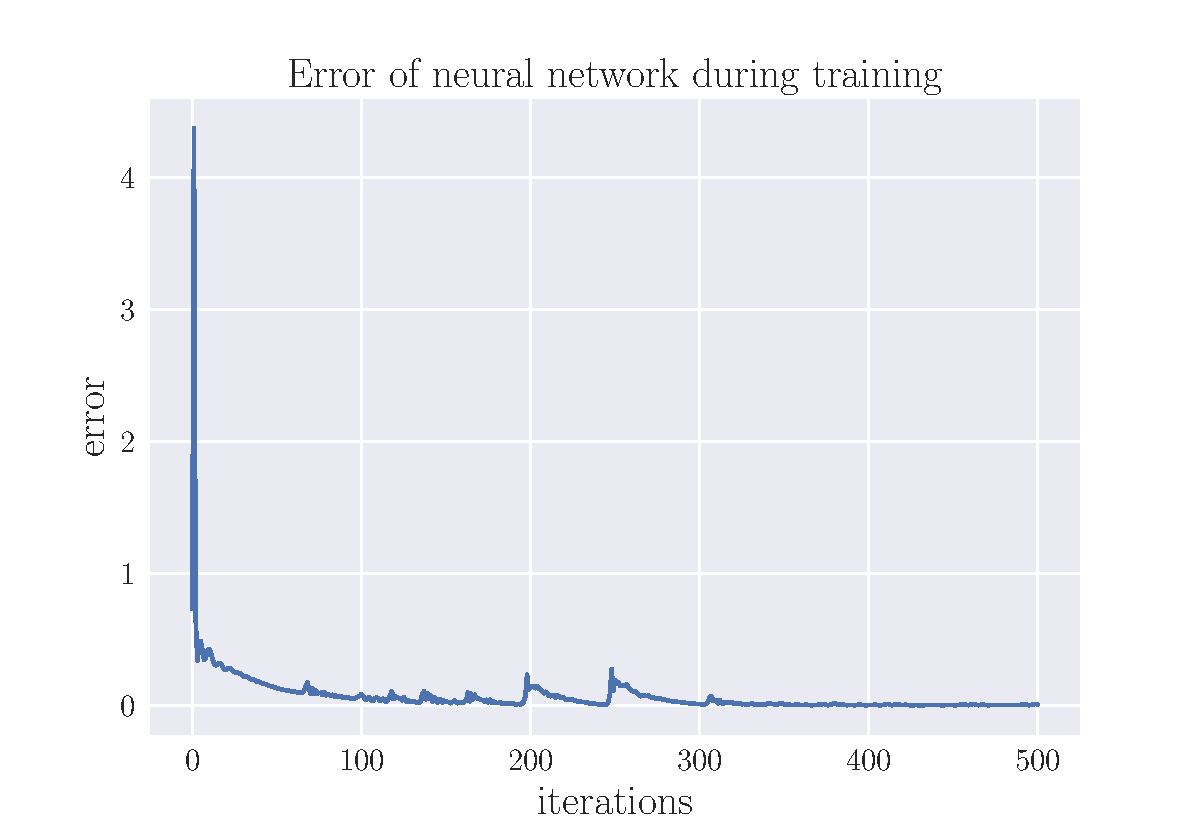
\includegraphics[scale=0.5]{../output/plots/NN_diffusion_error_40000}
	\caption{Residual of approximated solutions to the 1D diffusion equation. The neural network runs for 500 iterations, training on 40000 points.}
	\label{fig:error_NN_40000}
\end{figure}

The error of the neural network and the forward euler scheme are evaluated slightly different. In order to make a proper comparison, it is essential to accumulate the same amount of individual temporal errors to obtain an ultimate scalar measure for each method. This will represent the error of the approximated solution over the entire spatial and temporal domain. At each time level, the individual error is evaluated as the maximum absolute error between the approximated solution and the exact solution over the spatial domain. Hence, one must ensure that the same mesh resolutions are set.
\par A comparison of the total (accumulated) error is conducted using 20 points in space and 2000 points in time. This choice of resolution ensures stability for the forward euler scheme, and gives 40 000 training points for the neural network. Running these parameter settings for the neural network gives the total errors shown in Figure \ref{fig:error_NN_40000} for each iteration, while for the forward euler scheme it yields a total error of 0.083. The first run through the neural network gives an approximated solution with a total error of around 4, significantly worse than the solution proposed by forward euler. For later iterations, on the other hand, the error decreases tremendously and eventually converges towards zero.

\textcolor{red}{IS THIS THE RIGHT WAY TO COMPARE ERROR ??}
 

\section{Discussion}
\subsection*{Potential for solving differential equations}
The forward euler method and neural networks are two quite different methods for solving differential equations. The former relies on discretization of the derivative to arrive at an explicit recursive set of equations to solve for each time step. The latter uses the residual error from the approximation as a basis for backpropagation to update weights and biases to improve the approximation to the actual solution. Figure \ref{fig:error_NN_40000} visualizes how bad the approximated solution of the initial run of the neural network is. Just after a few iterations though, the error decreases tremendously and goes below 0.083 (which is the total error obtained from forward euler) after around 100 iterations. After this, the total error fluctuates mildly but eventually converges towards zero.
 
\par The forward euler method clearly has an advantage in its simple recursive formula and fast computation time. The proposed solution is calculated within a few milliseconds, with a total error of only 0.083. On the other hand, it is limited by a stability requirement in order to produce realistic results. This effectively puts a restriction on applicable mesh resolutions.

\par A notable drawback of the neural network is the demanding training process. To compute an approximated solution of \ref{eq:diffusion_equation_1D} requires calculating gradients and accumulating chained derivatives backwards through the hidden layers. This is a significantly larger computational effort than calculating the simple recursive formula of the forward euler scheme. As a result, the neural network suffers from a large computational runtime. Particularly, simulating for 40 000 training points takes about 3 minutes. Still, if training sufficiently long, the neural network will produce a better solution than forward euler and eventually yield a near perfect approximation to the exact solution. 

\par The forward euler scheme has proven to obtain good accuracy on the numerical solution. However, forward euler has an inherent disadvantage in that it is conditionally unstable with stability criteria given by \ref{eq:stability}. In general it means that the forward euler scheme is not a stable method for solving differential equations as it requires that we carefully assign the mesh discretization steps. Neural networks are not limited to any kind of discretization. From the \textcolor{red}{universal approximation theorem} it follows that a neural network with at least one hidden layer is able to approximate a non-linear function to arbitrary accuracy. Neural networks benefit from good convergence properties. That is, given enough time to train it is able to approximate the actual solution of a differential equation with an error of approximately zero. Moreover, the neural network model \ref{eq:NN_model} has the additional flexibility in that the function $f$ can be tweaked to give a better initial guess of the solution. 
\par Overall, the method of choice for solving differential equations is a tradeoff between the accuracy of the approximated solution and the computational runtime. Forward euler is definitely the desired method if we want a quick representation of the solution. If the importance is how precise the representation is, a neural network is a better choice.


\section{Conclusion}

\bibliographystyle{plain}
\bibliography{refs}
\end{document}

